% Copyright 2009 by Tomasz Mazur
%
% This file may be distributed and/or modified in all ways.


\documentclass[xcolor=pdftex,t,11pt]{beamer}

%%%%%%%%%%%%%%%%%%%%%%%%%%%%%%%%%%
%       SET OPTIONS BELOW        %
%%%%%%%%%%%%%%%%%%%%%%%%%%%%%%%%%%

\usetheme[
% Toggle showing page counter
pagecounter=true,
%
% String to be used between the current page and the
% total page count, e.g. of, /, from, etc.
pageofpages=of,
%
% Defines the shape of bullet points. Available options: circle, square
bullet=circle,
%
% Show a line below the frame title. 
titleline=true,
%
% Set the style of the title page (true for fancy, false for standard)
alternativetitlepage=true,
%
% Institution logo for fancy title page.
% Comment out to remove the logo from the title page.
% IMPORTANT: THERE IS A BUG IN SOME VERSIONS OF PDFLATEX AND FONTS
% ON THE LOGOS ARE NOT RENDERED PROPERLY. IN SUCH A CASE ADD `2` 
% TO THE NAME OF THE LOGO, E.G. comlab2 INSTEAD OF comlab
%titlepagelogo=images/titlepage/ou,
%
% Department footer logo for fancy title page
% Comment out to remove the logo from the footer of the title page/
% IMPORTANT: THERE IS A BUG IN SOME VERSIONS OF PDFLATEX AND FONTS
% ON THE LOGOS ARE NOT RENDERED PROPERLY. IN SUCH A CASE ADD `2` 
% TO THE NAME OF THE LOGO, E.G. comlab2 INSTEAD OF comlab
%titlepagefooterlogo=images/titlepage/comlab,
%
% Institution/department logo for ordinary slides
% Comment this line out to remove the logo from all the pages.
% Available logos are: ou, comlab, comlabinline, comlabou
% IMPORTANT: THERE IS A BUG IN SOME VERSIONS OF PDFLATEX AND FONTS
% ON THE LOGOS ARE NOT RENDERED PROPERLY. IN SUCH A CASE ADD `2` 
% TO THE NAME OF THE LOGO, E.G. comlab2 INSTEAD OF comlab
%ordinarypageslogo=TU-Signet,
%
%
% Add watermark in the bottom right corner
%watermark=<filename>,
%
% Set the height of the watermark.
%watermarkheight=100pt,
%
% The watermark image is 4 times bigger than watermarkheight.
%watermarkheightmult=4,
]{Torino}

% Select color theme. Available options are:
% mininmal, greenandblue, blue, red
\usecolortheme{blue}

%Select different font themes.Available options are:
% default, serif, structurebold, structureitalicserif, structuresmallcapsserif
\usefonttheme{structurebold}

\usepackage{tikz}
\usepackage{pgf}

\pgfdeclareimage[height=6ex]{ou-logo}{images/ou}

\logo{\pgfuseimage{ou-logo}}

\usepackage{listings}

\lstset{language=C,
 basicstyle=\tiny,
 mathescape=true
 }

\usepackage{ifthen}

\usepackage{moreverb}
\usepackage{pgf}
\usepackage{tikz}
\usetikzlibrary{arrows, automata, shapes.multipart, chains, positioning, fit}

\usepackage{pifont}
\newcommand{\xmark}{\ding{55}}

\usepackage{color}
\definecolor{light-gray}{gray}{0.80}

\usepackage{amsmath}
\usepackage{xspace}

\newcommand{\hpathlen}{\ensuremath{\mathit{pathLength}}\xspace}
\newcommand{\halloc}{\ensuremath{\mathit{new}}\xspace}
\newcommand{\hassign}{\ensuremath{\mathit{assign}}\xspace}
\newcommand{\hlookup}{\ensuremath{\mathit{lookup}}\xspace}
\newcommand{\hupdate}{\ensuremath{\mathit{update}}\xspace}
\newcommand{\halias}{\ensuremath{\mathit{alias}}\xspace}
\newcommand{\hisnull}{\ensuremath{\mathit{isNull}}\xspace}
\newcommand{\hispath}{\ensuremath{\mathit{isPath}}\xspace}
\newcommand{\hcircular}{\ensuremath{\mathit{circular}}\xspace}
%\newcommand{\id}{\ensuremath{\mathrm{id}}\xspace}
\newcommand{\hsubdivide}{\ensuremath{\mathit{subdivide}}\xspace}
\newcommand{\hfresh}{\ensuremath{\mathit{fresh}()}\xspace}

\newcommand{\defeq}{\ensuremath{\stackrel{\mathrm{def}}{=}}}

\newcommand{\kalashnikov}{{\sc Kalashnikov}\xspace}
\newcommand{\shakira}{{\sc Shakira}\xspace}


%%%%%%%%%%%%%%%%%%%%%%%%%%%%%%%%%%
%       PRESENTATION INFO        %
%%%%%%%%%%%%%%%%%%%%%%%%%%%%%%%%%%

\author{Matt Lewis}
\title{Precise Verification of C Programs}
%\subtitle{}
\institute{Oxford University}
\date{\today}

\begin{document}



%%%%%%%%%%%%%%%%%%%%%%%%%%%%%%%%%%
%       SLIDE DEFINITIONS        %
%%%%%%%%%%%%%%%%%%%%%%%%%%%%%%%%%%

\begin{frame}[plain]
  \titlepage
\end{frame}

\begin{frame}{Outline}
  \tableofcontents
\end{frame}

\section{Motivation and Thesis}

\begin{frame}{Motivation}
 Verifying C programs is hard, and most programs are incorrect.
 
 \vspace{1em}
 
 When using verification tools, I want something that can deal with programs that may be incorrect and can generate diagnostic counterexamples.
 
 \vspace{1em}
 
 I also want something that models C accurately.
 
 \vspace{1em}
 
 I don't want any false alarms, but I also don't want to miss any bugs.
\end{frame}

\begin{frame}{My Thesis}
 \begin{quote}
  It is possible to analyse C progams with loops, integer overflows and dynamically allocated data structures,
while at the same time generating no spurious warnings or claiming that unsafe programs are safe.
 \end{quote}
\end{frame}

\begin{frame}{Structure}
 The dissertation is split into two parts:
 
 \vspace{1em}
 
 \begin{enumerate}
  \item Underapproximate Loop Acceleration
  \item Second-Order Logic and Program Synthesis
 \end{enumerate}

\end{frame}


\section{Underapproximate Loop Acceleration}


\begin{frame}{Underapproximate Loop Acceleration}
 The first problem we tackle is \emph{finding deep bugs}.

 \vspace{1em}

 Our approach is to pick a \emph{single path} $\pi$ through a loop (thus underapproximating the loop) and
 then to find a \emph{closed form}, which captures the exact effects of executing $\pi$ a symbolic
 number $n$ times.

 \vspace{1em}

 We add this closed form back into the original program.  The new, accelerated program is non-deterministic,
 but bugs manifest themselves after far fewer iterations.
\end{frame}

\begin{frame}{Underapproximate Loop Acceleration}
 
 \vspace{2em}
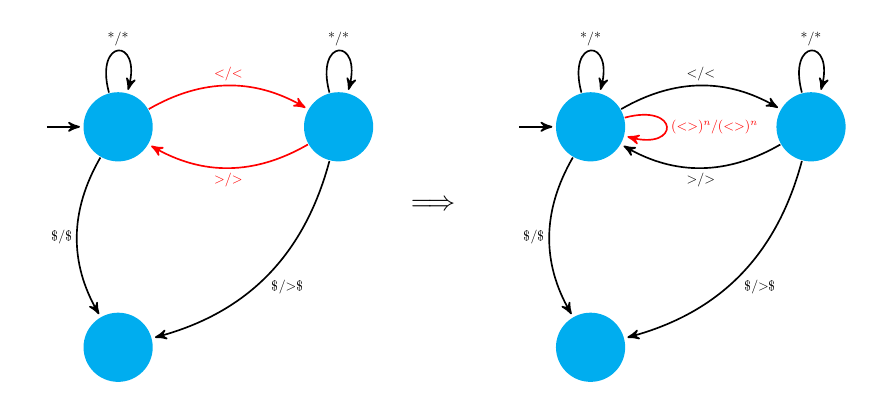
\begin{tikzpicture}[->,>=stealth',shorten >=1pt,auto,node distance=2.8cm,
 semithick, initial text=]
 \tikzstyle{every state}=[fill=cyan,draw=none,scale=1]
 
 \node[state,initial] (A) {};
 \node[state] (B) [right of=A] {};
 \node[state] (C) [below of=A]{};

 \begin{scope}[every node/.style={scale=0.5}]
  \path (A) edge    [loop above] node {*/*} (A)
        (A) edge    [bend left,color=red] node {\textless/\textless} (B)
        (B) edge    [loop above] node {*/*} (B)
        (B) edge    [bend left,color=red] node {\textgreater/\textgreater} (A)
        (A) edge    [bend right] node[swap] {\$/\$} (C)
        (B) edge    [bend left] node {\$/\textgreater\$} (C);
 \end{scope}

 \node at (4,-1) {$\Longrightarrow$};
 
 \node[state,initial] (A2) at (6, 0) {};
 \node[state] (B2) [right of=A2] {};
 \node[state] (C2) [below of=A2]{};

 \begin{scope}[every node/.style={scale=0.5}]
  \path (A2) edge    [loop above] node {*/*} (A2)
        (A2) edge    [loop right,color=red] node {$(<>)^n$/$(<>)^n$} (A2)
        (A2) edge    [bend left] node {\textless/\textless} (B2)
        (B2) edge    [loop above] node {*/*} (B2)
        (B2) edge    [bend left] node {\textgreater/\textgreater} (A2)
        (A2) edge    [bend right] node[swap] {\$/\$} (C2)
        (B2) edge    [bend left] node {\$/\textgreater\$} (C2);
 \end{scope}
\end{tikzpicture}
\end{frame}


\begin{frame}{Trace Automata}
 Underapproximate acceleration can find bugs, but it can't prove safety.

 \vspace{1em}

 To prove safety, we introduce \emph{trace automata}, which remove ``redundant'' traces
 from the accelerated program.
 
 \vspace{1em}
 
 The observation is that acceleration reduces the diameter of the program, and we can
 use trace automata to expose that diameter reduction to a bounded model checker.
\end{frame}


\section{Second-Order Logic and Program Synthesis}

\begin{frame}{Program Synthesis}
 We next turn our attention to \emph{program synthesis}.
 
 \vspace{1em}
 
 This is the problem of finding a program which meets some specification.
 
 \vspace{1em}
 
 We first show that finite state program synthesis is NEXPTIME-complete, and then build
 a finite state program synthesiser.
\end{frame}

\begin{frame}{Second-Order Logic}
 We can treat our program synthesiser as a decision procedure for \emph{finite, existential, second-order logic}.
 
 \vspace{1em}
 
 This logic is very rich.  We use it to directly build analysers which prove:
 
 \begin{itemize}
  \item Termination
  \item Non-termination
  \item Safety
  \item Existence of deep bugs
 \end{itemize}
\end{frame}

\begin{frame}{Modelling the Heap}
 In order to make the heap visible to our second-order logic solver, we need a
 theory of the heap which is decidable with a SAT solver.

 \vspace{1em}

 To do this, we model finite, singly linked lists as finite graphs.  We use
 \emph{homeomorphism classes} to find a small model property for the resulting logic.

 \vspace{1em}

 Our logic handles cyclic lists, arithmetic and unspecified sharing.  It also
 generates concrete counterexamples when a property does not hold.
\end{frame}

% 
% \section{Program Synthesis and Second-Order Logic}
% 
% \begin{frame}{Existential Second-Order Logic}
%  Second-order logic allows quantification over functions as well as ground terms.
%  
%  \vspace{1em}
%  
%  Existential second-order logic is a restriction where we can only existentially quantify over functions.
%  
% \end{frame}
% 
% \begin{frame}{Existential Second-Order Logic Example}
% The following is an existential second-order formula:
% 
%  \[
%   \exists F . \forall x . F(x) > x
%  \]
% 
%  When using Peano arithmetic as a background theory, this formula is satisfiable.  One satisfying assignment would be $F(x) = x + 1$.
% \end{frame}
% 
% \begin{frame}{Second-Order SAT}
%  A further restriction is to say that all the first-order variables are boolean propositions.  This
%  gives us the \emph{second-order SAT problem}.
% 
%  \vspace{1em}
% 
%  Second-order SAT is an extension of propositional SAT, where we are allowed to quantify
%  over functions.
%  
%  \vspace{1em}
%  
%  Second-order SAT is NEXPTIME-complete.
% \end{frame}
% 
% \begin{frame}{Using Second-Order SAT}
%  Second-order SAT is a very general problem and can be used for lots of problems, including:
%  
%  \begin{itemize}
%   \item Termination and non-termination
%   \item Safety invariants
%   \item Finding bugs without unwinding loops
%   \item Code refactoring
%   \item Code deobfuscation
%   \item Program synthesis
%   \item Concurrency
%  \end{itemize}
%  
%  Also since everything boils down to SAT, we can freely combine with any theory that is decidable in NP.
% \end{frame}
% 
% \begin{frame}{Solving Second-Order SAT}
%  To solve second-order SAT instances, we use a program synthesiser.
% 
%  \vspace{1em}
% 
%  The synthesiser finds programs computing each of the quantified functions.
% \end{frame}
% 
% \begin{frame}[fragile]{Example}
% Consider the following second-order SAT problem:
% 
%  \[
%   \exists F . \forall x . F(x) \neq x
%  \]
% 
% This formula is satisfiable.  To show this, our program synthesiser might generate the following program:
% 
% \begin{center}
% \begin{lstlisting}
% F(unsigned int x) {
%   unsigned int t1 = x + 1;
%   return t1;
% }
% \end{lstlisting}
% \end{center}
% \end{frame}
% 
% \section{Termination}
% 
% \begin{frame}{What Does a Termination Proof Look Like?}
% We prove that a program terminates by finding a \emph{ranking function}.
% 
% \vspace{1em}
% 
% If we have a transition relation $T$ and a loop guard $g$, a ranking function $R$
% must meet the following criteria:
% \begin{align}
%  \forall x, x' \cdot & g(x) \Rightarrow R(x) > 0 ~ \wedge \\
%                      & T(x, x') \Rightarrow R(x) > R(x')
% \end{align}
% 
% Or more generally, $R$ must be an order-homomorphism with a well-founded co-domain (aka an ordinal).
% 
% \vspace{1em}
% 
% We are therefore in the business of finding ranking functions.
% \end{frame}
% % 
% % \begin{frame}{Finding Ranking Functions}
% % Traditionally, people find ranking functions under some assumptions:
% % 
% % \begin{itemize}
% %  \item Programs are linear
% %  \item Ranking functions are linear
% %  \item Program variables are rationals
% % \end{itemize}
% % 
% % \vspace{1em}
% % 
% % With these assumptions in hand, one can deploy a very powerful piece of linear algebra: \emph{Farkas's lemma}.
% % 
% % This lemma makes light work of a ton of termination problems.
% % 
% % \vspace{1em}
% % 
% % But it's not for us.
% % \end{frame}
% 
% 
% \begin{frame}{Synthesing Ranking Functions}
% Our approach is to use \emph{program synthesis} to generate ranking functions.
% 
% \vspace{1em}
% 
% We're going to set up a program synthesis problem that will allow us to solve
% the following 2nd-order satisfaction problem:
% \begin{align*}
%  \exists R . \forall x, x' \cdot & g(x) \Rightarrow R(x) > 0 ~ \wedge \\
%                              & T(x, x') \Rightarrow R(x) > R(x')
% \end{align*}
% 
% \pause
% 
% \vspace{1em}
% 
% In other words: ``Is there a ranking function for my program?''
% 
% \end{frame}
% 
% \begin{frame}{Specifying a Ranking Function}
% Our program synthesiser needs a \emph{specification}, which takes the form of a C function.
% 
% \vspace{1em}
% 
% The specification function takes two arguments: a candidate program $P$ and an input $x$.
% If $P$ gives the correct output when fed $x$, our specification function returns true,
% otherwise it returns false.
% \end{frame}
% 
% \begin{frame}[fragile]{A Specification}
% 
% \vspace{-1em}
% 
% \begin{center}
% \begin{minipage}{.6\textwidth}
% \begin{lstlisting}[language=C++,basicstyle=\small]
% bool spec(prog_t *p, int x) {
%   int y = exec(p, x);
% 
%   if (y >= x)
%     return true;
%   else
%     return false;
% }
% \end{lstlisting}
% \end{minipage}
% \end{center}
% 
% \pause
% 
% Two of the possible programs:
% 
% \begin{itemize}
%   \item[] \texttt{int f(int x) \{ return x; \}} 
%   \item[] \texttt{int f(int x) \{ return MAXINT; \}}
% \end{itemize}
% 
% \end{frame}
% 
% \begin{frame}[fragile]{Specifying a Ranking Function}
% \vspace{-1em}
% 
% \begin{center}
% \begin{minipage}{0.6\textwidth}
% \begin{lstlisting}[language=c++,basicstyle=\small]
% int spec(prog_t *p, int x) {
%   int r1 = exec(p, x);
% 
%   if (g(x)) {
%     if (r1 <= 0)
%       return false;
% 
%     int y = body(x);
%     int r2 = exec(p, y);
%     
%     if (r1 <= r2)
%       return false;
%   }
%   
%   return true;
% }
% \end{lstlisting}
% \end{minipage}
% \end{center}
% \end{frame}
% 
% \iffalse
% 
% \section{Abstract Program Synthesis}
% \begin{frame}{The Synthesis Formula}
% Our high-level goal is to synthesise programs that meet some specification.
% 
% \pause
% 
% Abstractly, a program $P$ computes some function from an input set $I$ to an output set $O$:
% $$P : I \rightarrow O$$
% 
% \pause
% 
% A specification is a relation between inputs and outputs:
% $$\sigma \subseteq I \times O$$
% 
% \pause
% 
% The synthesis problem is to find a program that meets the specification on all inputs:
% $$\exists P . \forall x \in I . \sigma(x, P(x))$$
% \end{frame}
% \fi
% 
% \begin{frame}[fragile]{Solving the Synthesis Formula with CEGIS}
%  Solving second order formulae is hard.  Instead we'll alternately solve two \emph{first-order} formulae
%  in a refinement loop:
% 
%  \vspace{1cm}
%  
%   \begin{tikzpicture}[->,>=stealth',shorten >=1pt,auto,
%  semithick, initial text=]
% 
%   \matrix[nodes={draw, fill=none, scale=1, shape=rectangle, minimum height=1cm, minimum width=1.5cm},
%           row sep=2cm, column sep=3cm] {
%    \node (synth) {Synthesise};
%    &
%    \node (verif) {Verify}; %\\
%    %\node[draw=none] {};
%    &
%    \node[ellipse] (done) {Done}; \\
%   };
% 
%    \path
%     (synth) edge [bend left] node {Candidate program} (verif)
%     (verif) edge [bend left] node {Counterexample input} (synth)
%     (verif) edge node {Valid} (done);
%  \end{tikzpicture}
% \end{frame}
% 
% \begin{frame}{First-order Synthesis}
%  If we have some small set of test inputs $\{ x_0, \dots, x_N\}$, we can find a program that is correct on just that set:
% 
%  $$\exists P . \sigma(x_0, P(x_0)) \wedge \dots \wedge \sigma(x_N, P(x_N))$$
% \end{frame}
% 
% \begin{frame}{First-order Verification}
%  If we have some program $P$ that might be correct, we can check whether it is in fact correct:
%  
%  $$\exists x . \lnot \sigma(x, P(x))$$
%  
%  If this formula is \emph{satisfiable}, $P$ is \emph{not} correct and we have found an input on which it is incorrect.
%  We can add this input to our set of test inputs and loop back to synthesising a new program.
% \end{frame}
% 
% % \section{Program Synthesis}
% \iffalse
% \begin{frame}{Concrete Synthesis in C}
%  We're using C as an implementation language.  To do that we need:
%  
%  \begin{itemize}
%   \item A way of encoding programs as \emph{finite structures} in C.
%   \item A way of encoding the first-order synthesis and verification formulae in C.
%   \item A way of checking properties of C programs.
%  \end{itemize}
% \end{frame}
% 
% \begin{frame}[fragile]{Encoding Programs in C}
%  To encode the programs we will synthesise, we just make a very simple language and an interpreter for it.  Programs
%  in our language look like this:
% 
%  \vspace{0.7cm}
% 
% \begin{center}
% \begin{minipage}{0.3\linewidth}
% \begin{verbatimtab}
% t1 = neg x
% t2 = add t1 1
% return t2
% \end{verbatimtab}
% \end{minipage}
% \end{center}
% 
% \end{frame}
% 
% \fi
% 
% \begin{frame}{Complexity}
% By far the dominant factor in how long synthesis takes is the length of the shortest correct program.
% 
% \vspace{1em}
% 
% This is called the \emph{Kolmogorov complexity} of the function being computed.
% 
% \vspace{1em}
% 
% For termination, this gives us the property that our runtime doesn't depend very heavily
% on the size of the program we are analysing.  It is instead almost entirely determined by the
% size of the shortest program that computes a valid ranking function.
% \end{frame}
% 
% 
% \begin{frame}{Genetic Programming}
% The flip side of being so dominated by Kolmogorov complexity is that we
% get \emph{really slow} beyond about 4 instructions.
% 
% \vspace{1em}
% 
% It turns out that \emph{genetic programming} helps a lot beyond this threshold.
% \end{frame}
% 
% \begin{frame}{Genetic Programming}
% Genetic programming is an evolutionary search strategy, which aims to find a program
% that is ``fit'' according to some metric.
% 
% \vspace{1em}
% 
% It begins by generating a population of random programs.  This population is subjected to
% \emph{evolution} over a period of many generations.
% 
% \vspace{1em}
% 
% At each generation, each individual's fitness is evaluated.  The fitter an individual is,
% the greater its chance of breeding.
% 
% When two programs breed, their code is combined in some way (the crossover operation) and
% the resulting child may be randomly modified (the mutation operator).  This child is copied
% into the next generation.
% \end{frame}
% 
% \begin{frame}{Genetic Programming Synthesis}
% To use genetic programming for synthesis, we need to fix a useful fitness metric.
% 
% \vspace{1em}
% 
% For our purposes, we say that if a program meets the specification on $n$ test vectors, its
% fitness is $n$.
% 
% Whenever we add a new test vector, we continue genetic programming with the most recent population
% (the one that produced the most recent candidate program).  This is called \emph{incremental evolution}
% and gives us a big speedup.
% 
% \vspace{1em}
% 
% Once we've found a program that passes all the tests, we return it and continue round the CEGIS
% loop.
% \end{frame}
% 
% \begin{frame}[fragile]{Oh, And One More Thing}
% Does this terminate?  If so, what's the ranking function?
% 
% \begin{lstlisting}[basicstyle=\normalsize]
% while (x > 0 && y > 0 && z > 0) {
%   if (y > x) {
%     y = z;
%     x = nondet();
%     z = x - 1;
%   } else {
%     z = z - 1;
%     x = nondet();
%     y = x - 1;
%   }
% }
% \end{lstlisting}
% \end{frame}
% 
% 
% % \section{Advanced Topics}
% \begin{frame}{Conditional Termination}
% 
% \begin{align*}
% \exists I, R \cdot \forall x, x' \cdot & P(x, x') \Rightarrow & I(x') \\
%                                        & I(x) \wedge g(x) \wedge T(x, x') \Rightarrow & R(x) > 0 ~ \wedge \\
%                                        & & R(x) > R(x') ~ \wedge \\
%                                        & & I(x')
% \end{align*}
% \end{frame}
% 
% \begin{frame}{Sequential Loops}
% \begin{align*}
% \exists I_1, I_2, R \cdot \forall x, x' \cdot & P(x, x') \Rightarrow & I_1(x') \\
%                                               & I_1(x) \wedge g_1(x) \wedge T_1(x, x') \Rightarrow & I_1(x') \\
%                                               & I_1(x) \wedge \lnot g_1(x) \Rightarrow & I_2(x) \\
% 					      & I_2(x) \wedge g_2(x) \wedge T_2(x, x') \Rightarrow & R(x) > 0 ~ \wedge \\
% 					      & & R(x) > R(x') ~ \wedge \\
% 					      & & I_2(x')
% \end{align*}
% \end{frame}
% 
% 
% \begin{frame}{Some Combinatorics}
% A terminating program corresponds to a \emph{labelled partial order} on $2^k$ states.
% 
% \vspace{.7em}
% 
% Counting partial orders on a finite set turns out to be very hard (it's an open problem!).  However, asymptotics are known:
% \begin{align*}
%  P_n & = \left(1 + O \left( \frac{1}{n} \right) \right) \left( \sum_{i=1}^n \sum_{j=1}^{n-1} \binom{n}{i} \binom{n-i}{j} (2^i - 1)^j (2^j - 1)^{n - i - j}\right) \\
%      & \sim O\left( 2^k \right)
% \end{align*}
% 
% \end{frame}
% 
% \begin{frame}{More Combinatorics}
% Linear functions on bitvectors correspond to \emph{permutations} of the natural ordering on bitvectors.
% 
% \vspace{1em}
% 
% There are $2^{2k}$ linear functions (although only half of these permute the full space, cf. generators of the group $2^k$).
% 
% \vspace{1em}
% 
% Each of these functions can show that each of the \emph{unlabelled} partial orders terminates.
% 
% The number of unlabelled partial orders over an $n$ element set is related to the number of labelled partial orders as:
% 
% $$p_n \sim {P_n \over n!}$$
% \end{frame}
% 
% \begin{frame}{The Combinatorial Payoff}
% Since there are $P_n$ terminating functions, and each of the $n^2$ linear functions can prove that
% $p_n \sim {P_n \over n!}$ functions terminate, we can compute the probability that a random terminating
% function can be proved to terminate with a linear argument:
% 
% $${2^k \times 2^k \over {2^k}!} \sim {1 \over {2^k}!}$$
% 
% \pause
% 
% \vspace{1em}
% 
% This number is very small, which to some degree justifies our aim of moving beyond linear ranking functions.
% 
% \end{frame}
% 
% \section{Heap}
% 
% \begin{frame}[fragile]{Heaps of Singly Linked Lists}
% We would like to use second-order logic to analyse programs using the heap.  To do so, we need a
% heap theory with a decision procedure in NP that we can combine with arithmetic.
% 
% \pause
% 
% We will restrict ourselves to singly linked lists with lengths, but no data.
% 
% 
% \pause 
% 
% Lists can have (unspecified) cycles and sharing, for example:
% 
% \begin{center}
% \begin{tikzpicture}
%   %\node at (-.75,.25) {$h:$};
% 
%   \node (n1) {$\bullet$};
%   \node (n2) [below of=n1] {$\bullet$};
%   \node (n3) [right of=n1] {$\bullet$};
%   \node (n4) [right of=n3] {$\bullet$};
%   \node (n5) [right of=n4,above of=n4] {$\bullet$};
%   \node (n6) [below of=n4] {$\bullet$};
%   \node (x) [left of=n2] {$x$};
%   \node (y) [right of=n5] {$y$};
%   \node (z) [left  of=n1] {$z$};
%   \node (null) [right=2em of n6] {\bf null};
% 
%   \path[draw,->] (n1) edge (n3)
% 		 (n2) edge (n3)
% 		 (n3) edge (n4)
% 		 (n4) edge[bend right=45] (n5)
% 		 (n5) edge[bend right=45] (n4);
% 
%   \path[dashed,->] (x) edge (n2)%
% 		   (y) edge (n5)%
% 		   (z) edge (n1)%
% 		   (null) edge (n6);
%  \end{tikzpicture}
% \end{center}
% \end{frame}
% 
% \begin{frame}[fragile]{Heap Transformers}
% \only<1>{
% x = y$\rightarrow$next
% 
% \begin{center}
%  \begin{tikzpicture}
%   \node (n1) {$\bullet$};
%   \node [right of=n1] (n2) {$\bullet$};
%   \node (n3) [right of=n2] {$\bullet$};
% 
%   \node (y) [below=1em of n1] {$y$};
%   \node (x) [right of=y] {$x$};
%   \node (null) [right of=x] {\bf null};
% 
%   \path[draw, ->] (n1) edge (n2) (n2) edge (n3);
%   \path[dashed,->] (x) edge (n3) (y) edge (n1) (null) edge (n3);
% 
%   \node (mid) [below right = .5em and 1em of n3] {$\Rightarrow$};
% 
%   \node [above right = .5em and 1em of mid] (m1) {$\bullet$};
%   \node (m2) [right of = m1] {$\bullet$};
%   \node (m3) [right of = m2] {$\bullet$};
% 
%   \node (y) [below=1em of m1] {$y$};
%   \node (x) [right of=y] {$x$};
%   \node (null) [right of=x] {\bf null};
% 
%   \path[draw, ->] (m1) edge (m2) (m2) edge (m3);
%   \path[dashed,->] (x) edge (m2) (y) edge (m1) (null) edge (m3);
% \end{tikzpicture}
% \end{center}
% }
% 
% \only<2>{
% x = new()
% 
% \begin{center}
% \begin{tikzpicture}[shorten >=1pt,auto]
%   \node (n1) {$\bullet$};
%   \node (n2) [right of=n1] {$\bullet$};
%   \node (n3) [right of=n2] {$\bullet$};
% 
%   \node (x) [below of=n1] {$x$};
%   \node (null) [below of=n3] {\bf null};
% 
%   \path[draw, ->] (n1) edge (n2)
%                   (n2) edge (n3);
%   \draw[dashed,->] (x) to (n1);
%   \draw[dashed,->] (null) to (n3);
% 
%   \node [below right of=n3] (mid) {$\Rightarrow$};
% 
%   \node (m1) [above right of=mid]{$\bullet$};
%   \node (m2) [right of=m1] {$\bullet$};
%   \node (m3) [right of=m2] {$\bullet$};
%   \node (m4) [below of=m2] {$\bullet$};
% 
%   \node (x2) [below =1em of m4] {$x$};
%   \node (null) [right of=x2] {\bf null};
% each of these 
%   \path[draw, ->] (m1) edge (m2) (m2) edge (m3) (m4) edge (m3);
%   \draw[dashed,->] (x2) to (m4);
%   \draw[dashed,->] (null) to (m3);
%  \end{tikzpicture}
%  \end{center}
%  }
%  
%  \only<3>{
% x = y
% 
% \begin{center} 
%  \begin{tikzpicture}[shorten >=1pt,auto]
%   \node (n1) {$\bullet$};
%   \node (n2) [right of=n1] {$\bullet$};
%   \node (n3) [right of=n2] {$\bullet$};
%   \node (n4) [below=2em of n2] {$\bullet$};
% 
%   \node (y) [below=1em of n4] {$y$};
%   \node (x) [left of=y] {$x$};
%   \node (null) [right of=y] {\bf null};
% 
%   \path[draw, ->] (n1) edge (n2)
%                   (n2) edge (n3)
%                   (n4) edge (n3);
%   \path[dashed,->] (x) edge (n1)
%                    (y) edge (n4)
%                    (null) edge (n3);
% 
%   \node [below right of=n3] (mid) {$\Rightarrow$};
% 
%   \node (m1) [above right of=mid]{$\bullet$};
%   \node (m2) [right of=m1] {$\bullet$};
%   \node (m3) [right of=m2] {$\bullet$};
%   \node (m4) [below=2em of m2] {$\bullet$};
% 
%   \node (y2) [below=1em of m4] {$y$};
%   \node (x2) [left of=y2] {$x$};
%   \node (null) [right of=y2] {\bf null};
% 
%   \path[draw, ->] (m1) edge (m2)
%                   (m2) edge (m3)
%                   (m4) edge (m3);
%   \path[dashed,->] (x2) edge (m4)
%                    (y2) edge (m4)
%                    (null) edge (m3);
%  \end{tikzpicture}
%  \end{center}
%  }
% 
% \only<4>{
% x$\rightarrow$next = y
% 
% \begin{center}
%  \begin{tikzpicture}[shorten >=1pt,auto]
%   \node (n1) {$\bullet$};
%   \node (n2) [right of=n1] {$\bullet$};
%   \node (n3) [right of=n2] {$\bullet$};
%   \node (n4) [below=2em of n2] {$\bullet$};
% 
%   \node (y) [below=1em of n4] {$y$};
%   \node (x) [left of=y] {$x$};
%   \node (null) [right of=y] {\bf null};
% 
%   \path[draw, ->] (n1) edge (n2)
%                   (n2) edge (n3)
%                   (n4) edge (n3);
%   \path[dashed,->] (x) edge (n1)
%                    (y) edge (n4)
%                    (null) edge (n3);
% 
%   \node [below right of=n3] (mid) {$\Rightarrow$};
% 
%   \node (m1) [above right of=mid]{$\bullet$};
%   \node (m2) [right of=m1] {$\bullet$};
%   \node (m3) [right of=m2] {$\bullet$};
%   \node (m4) [below=2em of m2] {$\bullet$};
% 
%   \node (y2) [below=1em of m4] {$y$};
%   \node (x2) [left of=y2] {$x$};
%   \node (null) [right of=y2] {\bf null};
% 
%   \path[draw, ->] (m1) edge (m4)
%                   (m2) edge (m3)
%                   (m4) edge (m3);
%   \path[dashed,->] (x2) edge (m1)
%                    (y2) edge (m4)
%                    (null) edge (m3);
%  \end{tikzpicture}
% \end{center}
% }
% 
% \end{frame}
% 
% \begin{frame}[fragile]{Heap Observations}
% 
% \begin{center}
% \begin{minipage}[c]{.4\textwidth}
% \begin{tikzpicture}[>=stealth',shorten >=1pt,auto,scale=.8]
%   %\node at (-.75,.25) {$h:$};
% 
%   \node (n1) {$\bullet$};
%   \node (n2) [below of=n1] {$\bullet$};
%   \node (n3) [right of=n1] {$\bullet$};
%   \node (n4) [right of=n3] {$\bullet$};
%   \node (n5) [right of=n4,above of=n4] {$\bullet$};
%   \node (n6) [below of=n4] {$\bullet$};
%   \node (x) [below of=n2] {$x$};
%   \node (y) [right of=n5] {$y$};
%   \node (z) [above of=n1] {$z$};
%   \node (null) [below of=n6] {\bf null};
% 
%   \path[draw,->] (n1) edge (n3)
% 		 (n2) edge (n3)
% 		 (n3) edge (n4)
% 		 (n4) edge[bend right=45] (n5)
% 		 (n5) edge[bend right=45] (n4);
% 
%   \path[dashed,->] (x) edge (n2)%
% 		   (y) edge (n5)%
% 		   (z) edge (n1)%
% 		   (null) edge (n6);
%  \end{tikzpicture}
%  \end{minipage}
%  \begin{minipage}[c]{.4\textwidth}
%  \vfill
%  \begin{align*}
%  \hpathlen(x, y) & =  3 \\
%  \hispath(z, y) & = \text{true} \\
%  \hispath(x, z) & = \text{false} \\
%  \halias(x, z) & = \text{false} \\
%  \hisnull(x) & = \text{false} \\
%  \hcircular(y) & = \text{true}
%  \end{align*}
%  \vfill
%  \end{minipage}
% \end{center}
% \end{frame}
% 
% \begin{frame}[fragile]{The SLH Theory}
%  SLH is our theory of singly linked lists.  SLH formulae can contain arbitrary boolean combinations of the
%  predicates from the previous slides.
%  
%  For example:
%  
%  \[
%   h' = \halloc(h, x) \wedge \hisnull(h', x)
%  \]
% 
% \end{frame}
% 
% \begin{frame}{\shakira}
%  We built a decision procedure for SLH named \shakira, which checks that heaps don't lie.
% 
%  \pause 
% 
%  \shakira works by exploiting a small model property of SLH to build a SAT formula that is equisatisfiabile with the SLH formula.
% \end{frame}
% 
% 
% \begin{frame}[fragile]{Edge Subdivision}
% \begin{center}
%  \begin{tikzpicture}
%   \node (h) {$H:$};
% 
%   \node (n1) [below right =.1em and .1em of h] {$\bullet$};
%   \node (space) [right of=n1] {};
%   \node (n2) [right of=space] {$\bullet$};
% 
%   \node (x) [below of=n1] {$x$};
%   \node (null) [below of=n2] {\bf null};
% 
%   \path[draw, ->] (n1) to node[above] {3} (n2);
%   \path[dashed,->] (x) edge (n1)
%                    (null) edge (n2);
% 
%   \node (h2) [right=9em of h] {$H':$};
% 
%   \node (m1)[below right =.1em and .1em of h2] {$\bullet$};
%   \node (m2) [right of=m1] {$\bullet$};
%   \node (m3) [right of=m2] {$\bullet$};
% 
%   \node (x2) [below of=m1] {$x$};
%   \node (null2) [below of=m3] {\bf null};
% 
%   \path[draw, ->] (m1) edge node[above] {1} (m2)
%                   (m2) edge node [above] {2} (m3);
%   \path[dashed,->] (x2) edge (m1)
% 		   (null2) edge (m3);
%  \end{tikzpicture}
% \end{center}
% 
%  \vspace{1em}
%  $H'$ can be generated from $H$ by subdividing an edge.  We say $H'$ is a \emph{subdivision} of $H$.
% \end{frame}
% 
% 
% \begin{frame}[fragile]{Heap Homeomorphism}
%  
%  \begin{center}
%  \resizebox{\textwidth}{!}{
%  \begin{tikzpicture}
%   \node (h) {$H:$};
% 
%   \node (x) [below right =.1em and .1em of h] {$x$};
%   \node (y) [below of=x] {$y$};
%   
%   \node (n1) [right of=x] {$\bullet$};
%   \node (n2) [below of=n1] {$\bullet$};
% 
%   \path (n1) to node (mid) {} (n2);
% 
%   \node (n3) [right of=mid] {$\bullet$};
%   \node (n4) [right of=n3] {$\bullet$};
% 
%   \node (n5) [right of=n4] {$\bullet$};
%   \node (space2) [right of=n5] {};
%   \node (n6) [right of=space2] {$\bullet$};
% 
%   \path[->,draw] (n1) edge node [above] {1} (n3)
%                  (n2) edge node [below] {2} (n3)
%                  (n3) edge node [above] {4} (n4)
%                  (n4) edge node [above] {2} (n5)
%                  (n5) edge[bend right=70] node [below] {6} (n6)
%                  (n6) edge[bend right=70] node [above] {3} (n5);
% 
%   \path[->,dashed] (x) edge (n1)
%                    (y) edge (n2);
% 
%   \node (h2) [right=20em of h] {$H':$};
% 
%   \node (x2) [below right =.1em and .1em of h2] {$x$};
%   \node (y2) [below of=x2] {$y$};
% 
%   \node (m1) [right of=x2] {$\bullet$};
%   \node (m2) [below of=m1] {$\bullet$};
% 
%   \path (m1) to node (mid2) {} (m2);
% 
%   \node (m3) [right of=mid2] {$\bullet$};
%   \node (m4) [right of=m3] {};
% 
%   \node (m5) [right of=m4] {$\bullet$};
%   \node (space2) [right of=m5] {};
%   \node (m6) [right of=space2] {$\bullet$};
% 
%   \node (m7) [above of=space2] {$\bullet$};
% 
%   \path[->,draw] (m1) edge node [above] {1} (m3)
%                  (m2) edge node [below] {2} (m3)
%                  (m3) edge node [above] {6} (m5)
%                  (m5) edge[bend right=70] node [below] {6} (m6)
%                  (m6) edge[bend right=35] node [above] {1} (m7)
%                  (m7) edge[bend right=35] node [above] {2} (m5);
% 
%   \path[->,dashed] (x2) edge (m1)
%                    (y2) edge (m2);
% 
%   \node (s) [below right=7em and 8em of h] {$S:$};
% 
%   \node (x) [below right =.1em and .1em of s] {$x$};
%   \node (y) [below of=x] {$y$};
% 
%   \node (n1) [right of=x] {$\bullet$};
%   \node (n2) [below of=n1] {$\bullet$};
% 
%   \path (n1) to node (mid) {} (n2);
% 
%   \node (n3) [right of=mid] {$\bullet$};
%   \node (n4) [right of=n3] {$\bullet$};
% 
%   \node (n5) [right of=n4] {$\bullet$};
%   \node (space2) [right of=n5] {};
%   \node (n6) [right of=space2] {$\bullet$};
% 
%   \node (n7) [above of=space2] {$\bullet$};
% 
%   \path[->,draw] (n1) edge node [above] {1} (n3)
%                  (n2) edge node [below] {2} (n3)
%                  (n3) edge node [above] {4} (n4)
%                  (n4) edge node [above] {2} (n5)
%                  (n5) edge[bend right=70] node [below] {6} (n6)
%                  (n6) edge[bend right=35] node [above] {1} (n7)
%                  (n7) edge[bend right=35] node [above] {2} (n5);
% 
%   \path[->,dashed] (x) edge (n1)
%                    (y) edge (n2);
% % 
% %   \node (x) [below of=n1] {$x$};
% %   \node (null) [below of=n2] {\bf null};
% % 
% %   \path[draw, ->] (n1) to node[above] {3} (n2);
% %   \path[dashed,->] (x) edge (n1) 
% %                    (null) edge (n2);
% % 
% %   \node (h2) [right=9em of h] {$H':$};
% % 
% %   \node (m1)[below right =.1em and .1em of h2] {$\bullet$};
% %   \node (m2) [right of=m1] {$\bullet$};
% %   \node (m3) [right of=m2] {$\bullet$};
% % 
% %   \node (x2) [below of=m1] {$x$};
% %   \node (null2) [below of=m3] {\bf null};
% % 
% %   \path[draw, ->] (m1) edge node[above] {1} (m2)
% %                   (m2) edge node [above] {2} (m3);
% %   \path[dashed,->] (x2) edge (m1)
% %                    (null2) edge (m3);
%  \end{tikzpicture}
%  }
%  \end{center}
% 
%  Both $H$ and $H'$ can be subdivided to produce $S$.  We then say that $H$ and $H'$ are \emph{homeomorphic}.
% \end{frame}
% 
% \begin{frame}{SLH Has Small Models}
%  \begin{theorem}[Homeomorphism Preserves Models]
%   If two heaps are homeomorphic, they satisfy exactly the same SLH formulae.
%  \end{theorem}
% 
%  \begin{theorem}[Homeomorphisms Can Be Small]
%   Every homeomorphism class has a least element, which has no more than $2P$ nodes ($P$ is the number of program variables).
%  \end{theorem}
% 
%  From this it follows that SLH has small models -- we only need to check models up to size $2P$.
% \end{frame}
% 
% 
% \begin{frame}[fragile]{Fin}
% 
% \begin{center}
% \includegraphics[width=.7\textwidth]{sloth.jpg}
% 
% \Huge
%  Thank you!
% \end{center}
% 
% \end{frame}


\end{document}